% Drawing 83/03-3 -- folder 83, batch 03, archive page 53 (PDF page 54).
% Transcription: un losange formé de deux triangles ayant l'arête $a$ en commun, avec une flèche courbe au-dessus : « carré $Q_{\mathcal I}$ »
% Kind: rhombus of two triangles with a curved arrow. Method 2 (schematic redraw from the facsimile). Status: ok.
% Notes: Two triangles sharing the horizontal edge a (thick), drawn heavily; a curved arrow over the top vertex. The edge label a and the caption "carre Q_I" are written beside it ("Car..." to the right); a is placed on the shared edge after the transcription.
% Coordinates: 1 unit = 1 mm = 1/100 of the crop width (bbox in page fractions: [0.18, 0.28, 0.3, 0.35]).
% Redrawn by Claude (claude-opus-5-5), issue #73, 2026-11-07; not checked by a human; not compiled (no TeX in the session).
% Rights: reproduces part of the work -- behind RENDER_TRANSCRIPTS, never published by itself.
\documentclass[tikz,border=3pt]{standalone}
\usepackage{amsmath,amssymb}
\usetikzlibrary{patterns,arrows.meta}
\tikzset{pencil/.style={black!45}, struck/.style={black!35}, mark/.style={circle,draw,inner sep=1.3pt}, pt/.style={circle,fill,inner sep=0.9pt}, opt/.style={circle,draw,fill=white,inner sep=1.1pt}}
\begin{document}
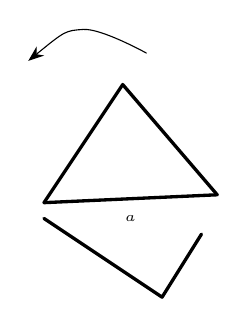
\begin{tikzpicture}[x=1mm,y=1mm,line cap=round,line join=round,font=\scriptsize]
\draw[very thick] (28,-34) -- (38,-19) -- (50,-33);
\draw[very thick] (28,-34) -- (50,-33);
\draw[very thick] (28,-36) -- (43,-46) -- (48,-38);
\draw[{Stealth[length=2mm]}-] plot[smooth, tension=0.55] coordinates {(26,-16) (33,-12) (41,-15)};
\node[inner sep=1pt] at (39,-36) {\tiny $a$};
\end{tikzpicture}
\end{document}
